\chapter{Tensorflow基础}
\section{Tensorflow基础函数}
\subsection{Variable}
\begin{python}
#tensorflow 1.2.1
import tensorflow as tf
var = tf.Variable(0)
add_operation = tf.add(var,1)
update_operation = tf.assign(var,add_operation)
with tf.Session() as sess:
    sess.run(tf.global_variables_initializer())
    for _ in range(3):
        sess.run(update_operation)
        print(sess.run(var))
\end{python}
\subsection{placeholder}
\begin{python}
#tensorflow 1.2
import tensorflow as tf
x1 = tf.placeholder(dtype=tf.float32,shape=None)
y1 = tf.placeholder(dtype=tf.float32,shape=None)
z1 = x1+y1
x2 = tf.placeholder(dtype=tf.float32,shape=[2,1])
y2 = tf.placeholder(dtype=tf.float32,shape=[1,2])
z2 = tf.matmul(x2,y2)
with tf.Session() as sess:
    z1_value = sess.run(z1,feed_dict={x1:1,y1:2})
    z1_value,z2_value = sess.run([z1,z2],feed_dict={x1:1,y1:2,x2:[[2],[2]],y2:[[3,3]]})
    print(z1_value)
    print(z2_value)
\end{python}
\subsection{batch normalization}

\begin{itemize}
	\item[\S] 数据x为Tensor。
\item mean:为x的均值,也是一个Tensor。
\item var:为x的方差,也为一个Tensor。
\item offset:一个偏移,也是一个Tensor。
\item scale:缩放倍数,也是一个Tensor。
\item variable\_epsilon,一个不为0的浮点数。
\item name:操作的名字,可选。
\end{itemize}
batch normalization计算方式是:
\begin{gather}
x = (x-\bar{x})/\sqrt{Var(x)+variable_{epsilon}}\\
x = x\times scale+offset\\
\end{gather}
\begin{gather}
\text{均值}:\bar{x} = \frac{1}{m}\Sigma_{i=1}^{m}x_i\\
\text{方差}:\sigma^2 = \frac{1}{m}\Sigma_{i=1}^m(x_i-\bar{x})
\end{gather}
\subsection{常见的的激活函数}
\begin{itemize}
\item relu
\item sigmoid
\item tanh
\item elu
\item bias\_add
\item relu6
\item softplus
\item softsign
\end{itemize}
\section{relu函数}
\subsection{relu}
relu函数在自变量x小于0时值全为0,在x大于0时,值和自变量相等。
\begin{python}
import tensorflow as tf 
import matplotlib.pyplot as plt 
x = tf.linspace(-10.,10.,100)
y = tf.nn.relu(x)
with tf.Session() as sess:
	[x,y] = sess.run([x,y])
plt.plot(x,y,'r',6,6,'bo')
plt.title('relu')
ax = plt.gca()
ax.annotate("",
            xy=(6, 6), xycoords='data',
            xytext=(6, 4.5), textcoords='data',
            arrowprops=dict(arrowstyle="->",
                            connectionstyle="arc3"),
            )
ax.annotate("",xy=(6,6),xycoords='data',
            xytext=(10, 6), textcoords='data',
            arrowprops=dict(arrowstyle="->",
                            connectionstyle="arc3"),
	  	   
)
ax.grid(True)
plt.xlabel('x')
plt.ylabel('relu(x)')
plt.savefig('relu.png',dpi = 600)
\end{python}
\subsection{relu6}
relu6函数和relu不同之处在于在x大于等于6的部分值保持为6。
\begin{python}
import tensorflow as tf 
import matplotlib.pyplot as plt 
x = tf.linspace(-10.,10.,100)
y = tf.nn.relu6(x)
with tf.Session() as sess:
	[x,y] = sess.run([x,y])
plt.plot(x,y,'r',6,6,'bo')
plt.title('relu6')
ax = plt.gca()
ax.annotate("",
            xy=(6, 6), xycoords='data',
            xytext=(6, 4.5), textcoords='data',
            arrowprops=dict(arrowstyle="->",
                            connectionstyle="arc3"),
            )
ax.grid(True)
plt.xlabel('x')
plt.ylabel('relu6(x)')
plt.savefig('relu6.png',dpi = 600)
\end{python}
\begin{figure}[H]
\centering
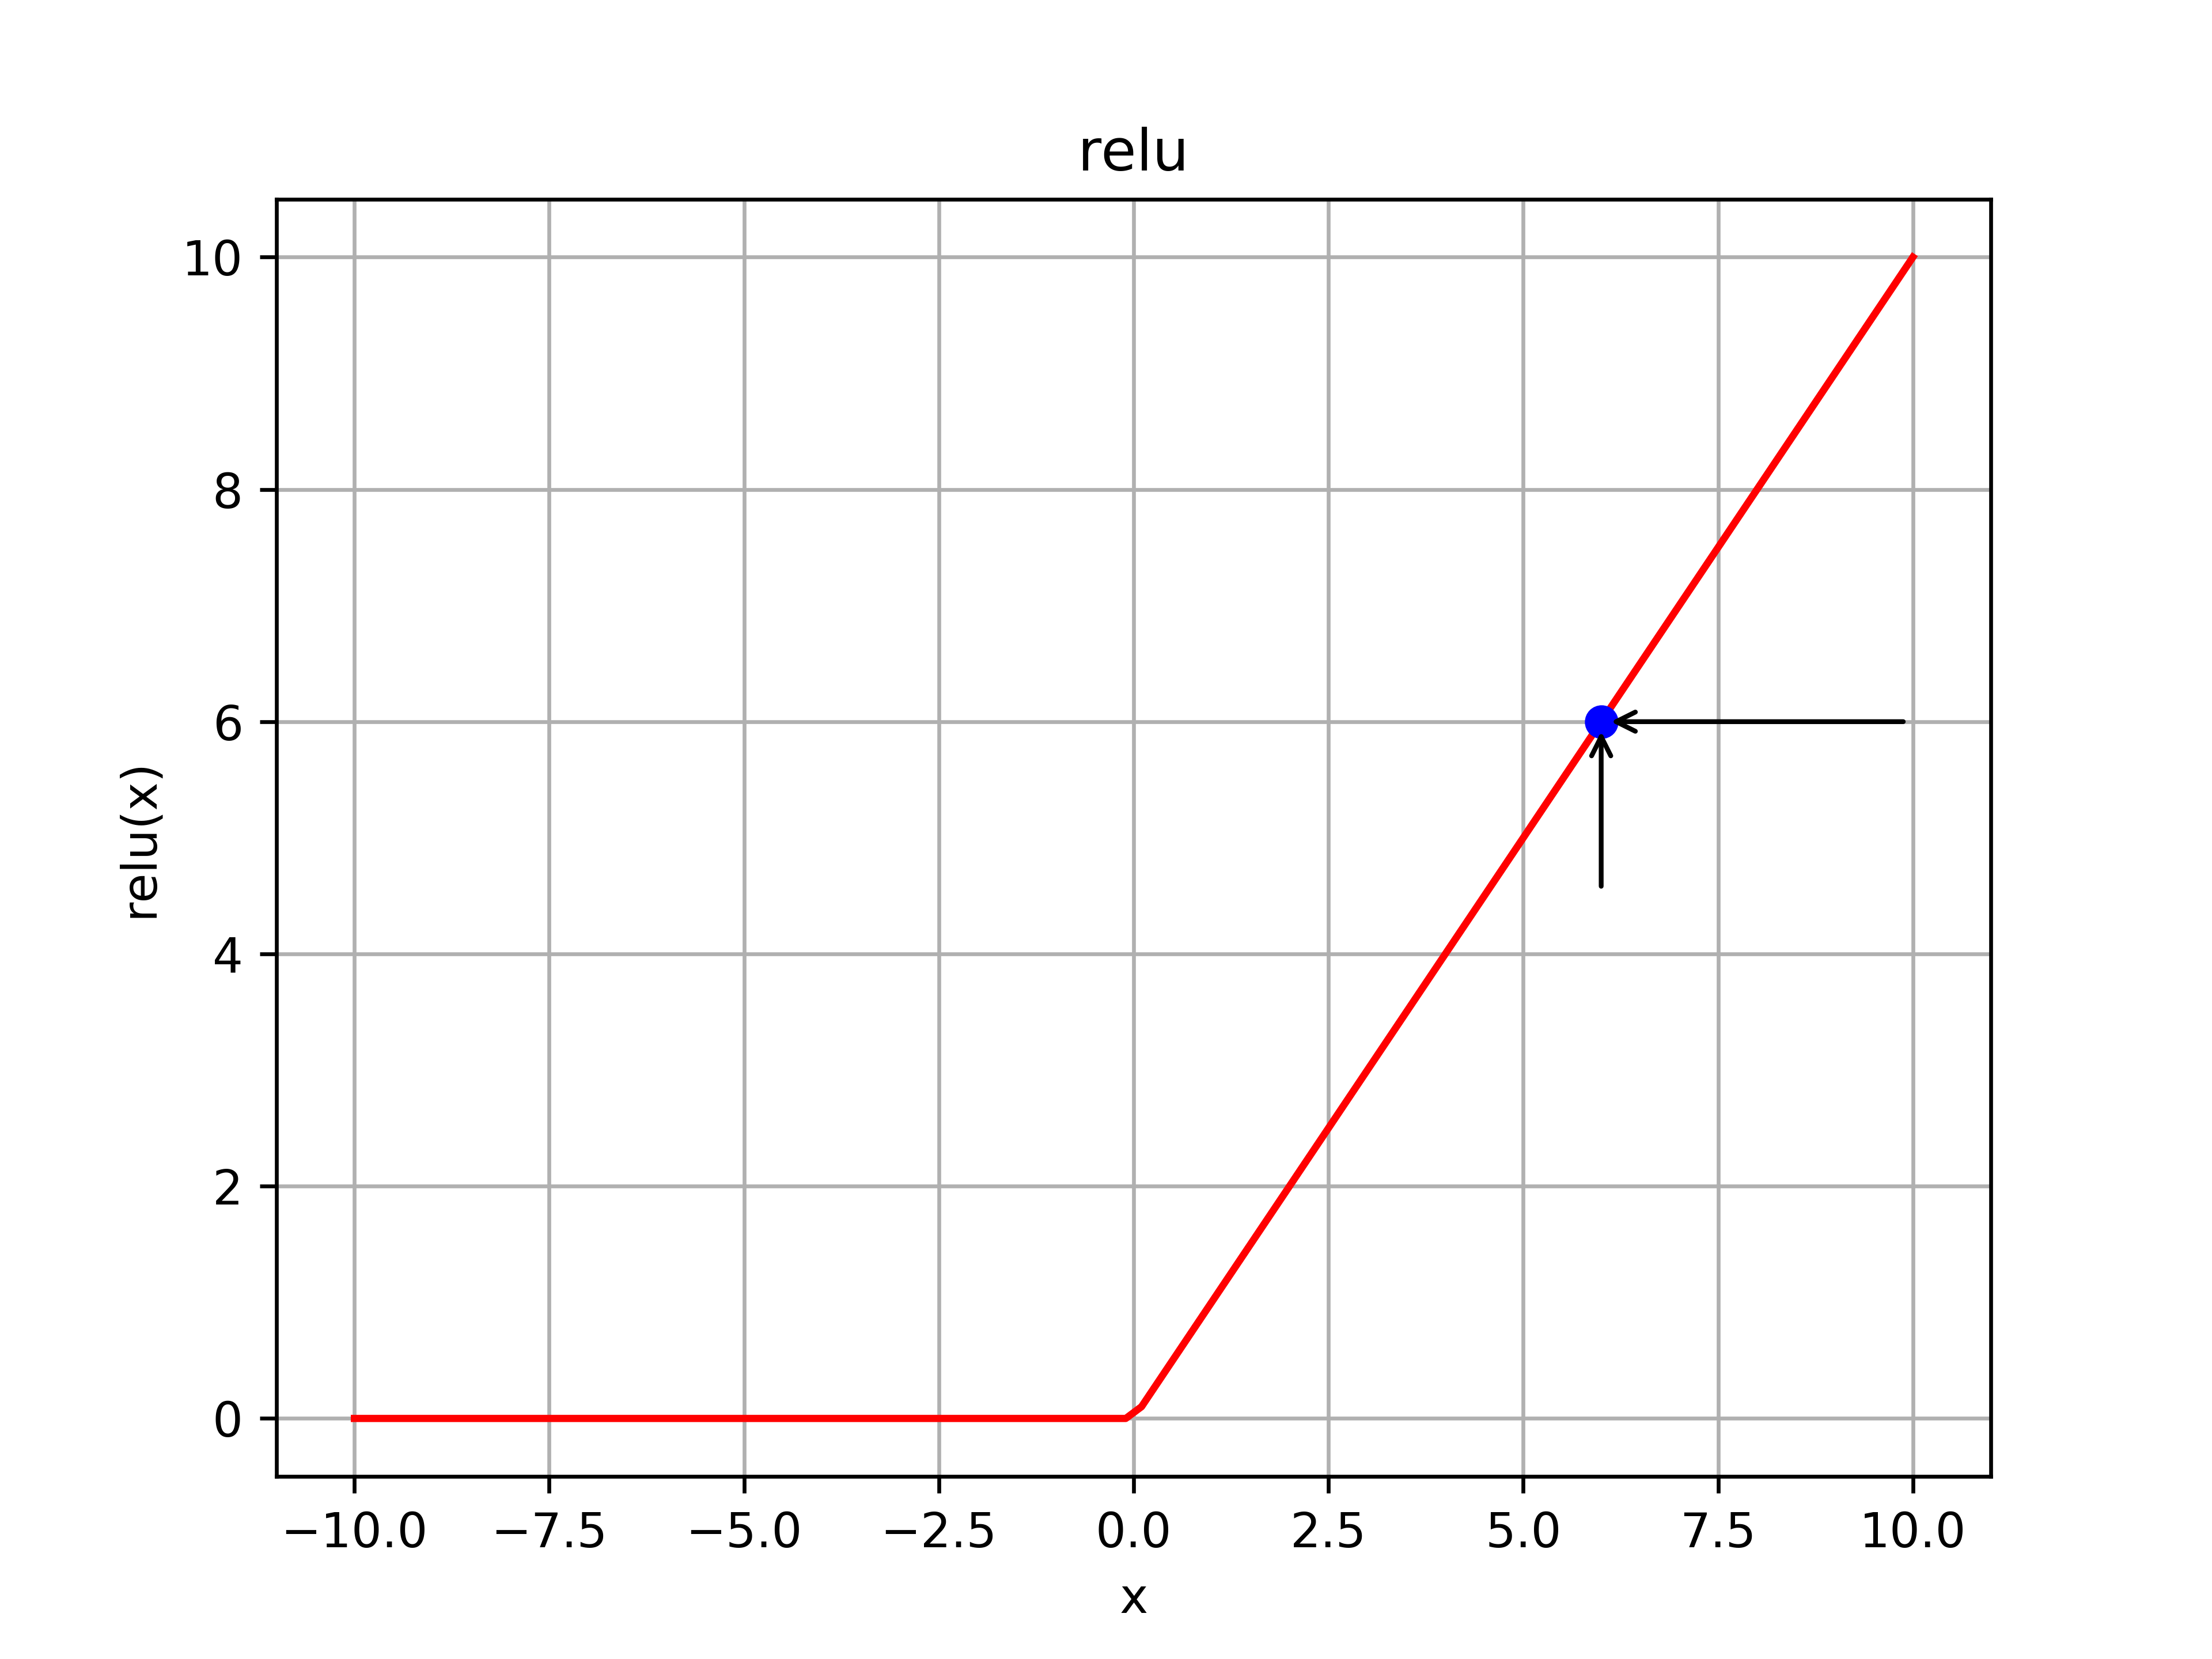
\includegraphics[scale=0.8]{./pic/chapter1/relu.png}
\caption{relu}
\end{figure}
\begin{figure}[H]
\centering
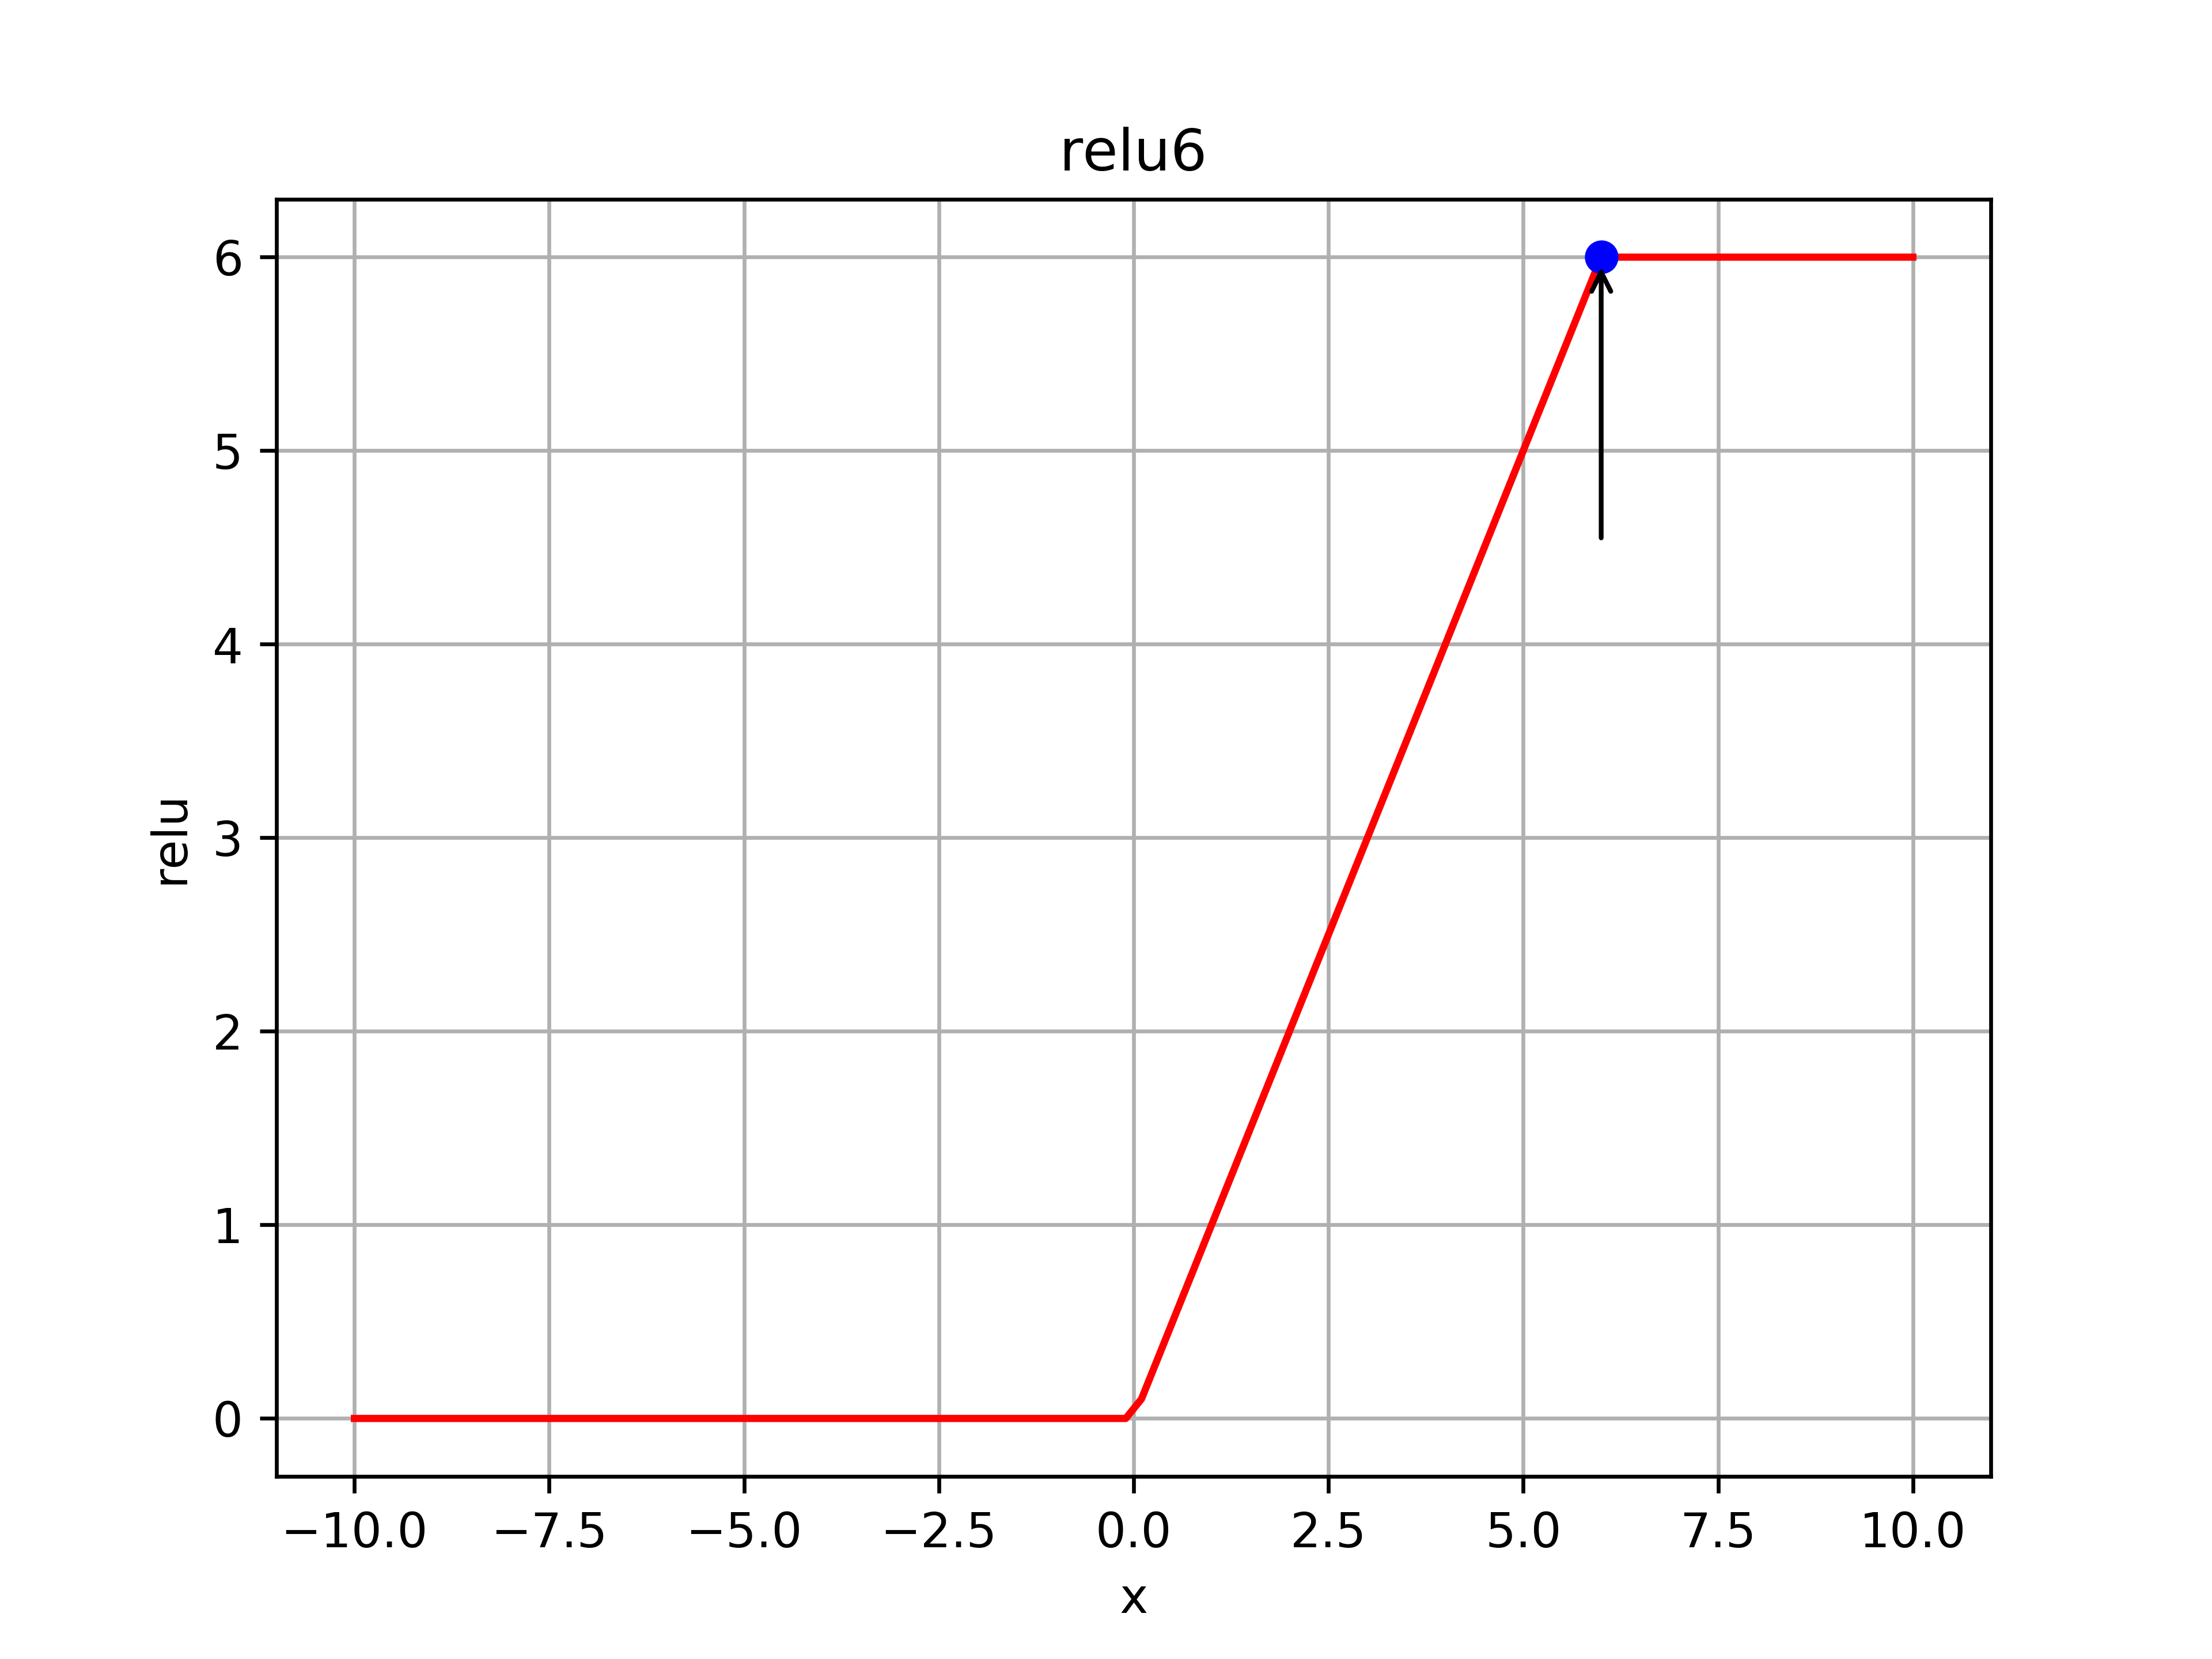
\includegraphics[scale=0.8]{./pic/chapter1/relu6.png}
\caption{relu6}
\end{figure}

\subsection{sigmoid}
\begin{python}
import tensorflow as tf 
import matplotlib.pyplot as plt 
import matplotlib.patches as mpatches
x = tf.linspace(-10.,10.,100)
y1 = tf.nn.sigmoid(x)
y2 = tf.nn.tanh(x)
red_patch = mpatches.Patch(color = 'red',label = 'sigmoid')
blue_patch = mpatches.Patch(color = 'blue',label = 'tanh')
with tf.Session() as sess:
	[x,y1,y2] = sess.run([x,y1,y2])
plt.plot(x,y1,'r',x,y2,'b')
ax = plt.gca()
ax.annotate(r"$tanh(x) = \frac{1-^{-2x}}{1+e^{-x}}$",
	   xy=(0,0),xycoords="data",
	   xytext=(1,0),textcoords="data",
	   arrowprops=dict(arrowstyle="->",
	   connectionstyle="arc3"),
)
ax.annotate(r"$sigmoid(x) = \frac{1}{1+e^{-x}}$",
	   xy=(0,0.5),xycoords="data",
	   xytext=(1,0.5),textcoords="data",
	   arrowprops=dict(arrowstyle="->",
	   connectionstyle="arc3"),
)
plt.xlabel('x')
plt.grid(True)
plt.legend(handles = [red\_patch,blue\_patch])
plt.savefig('activate.png',dpi=600)
\end{python}
\begin{figure}[H]
\centering
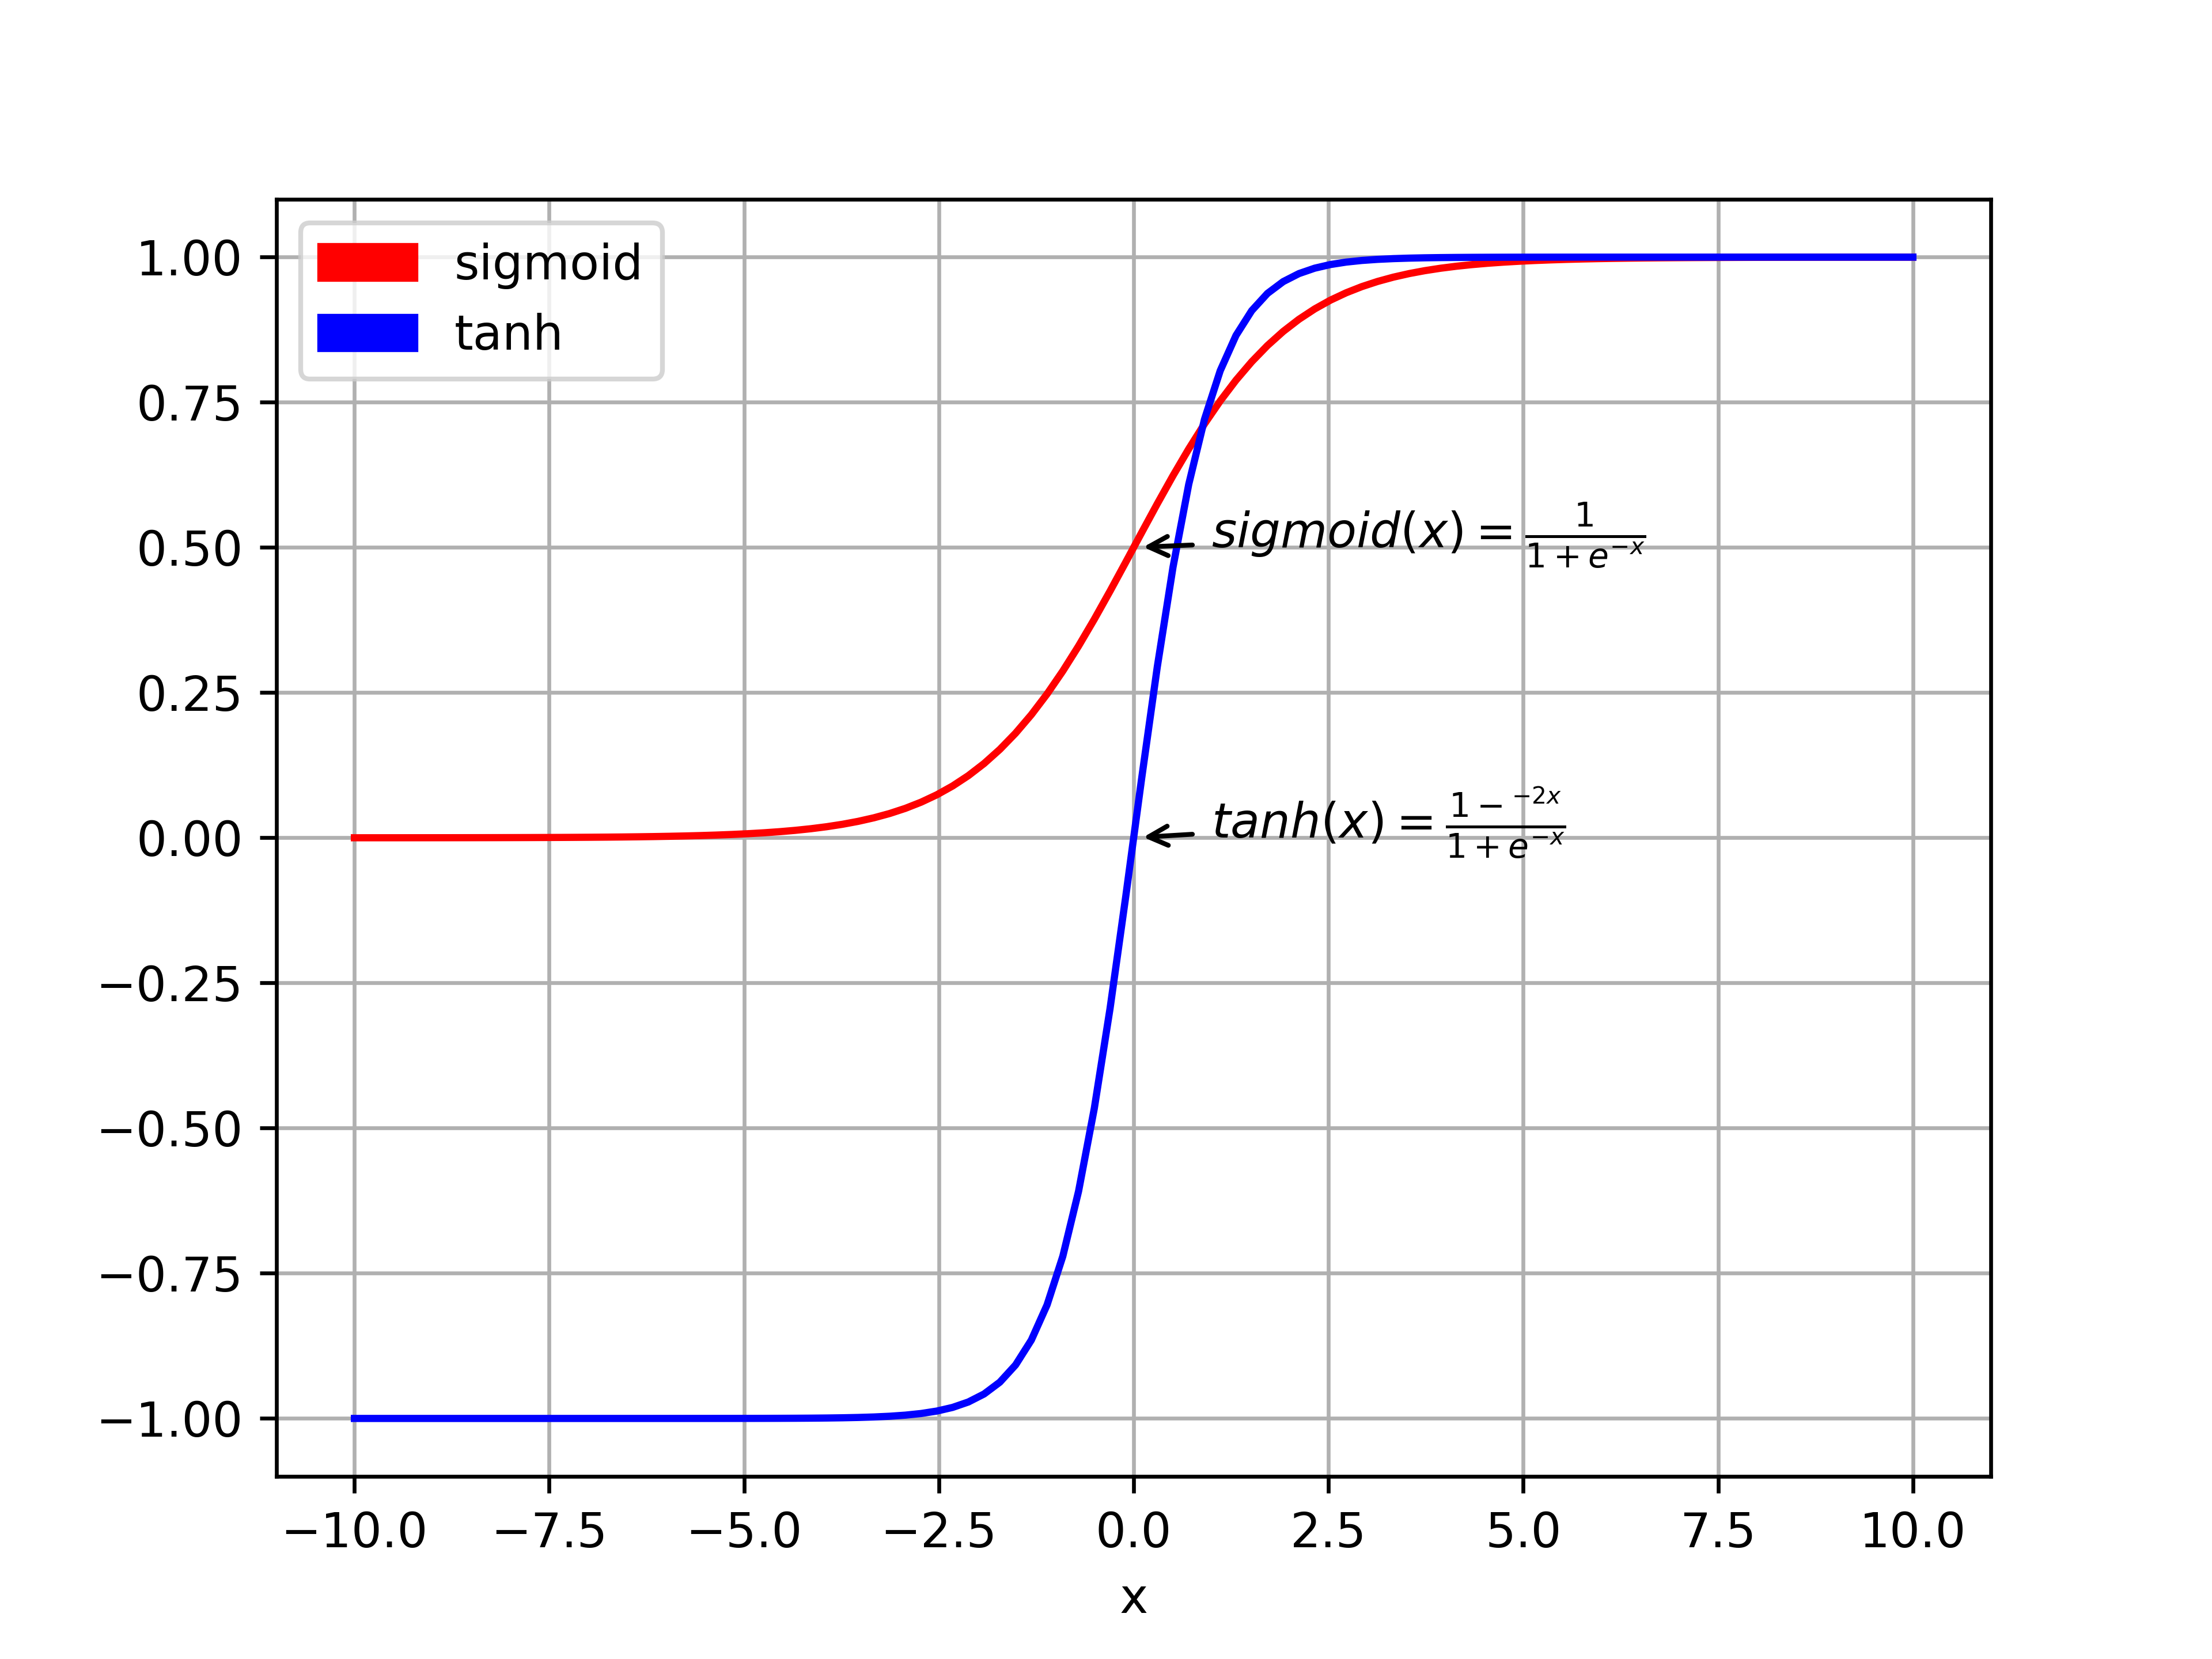
\includegraphics[scale=0.8]{./pic/chapter1/activate_fun.png}
\caption{activate\_fun}
\end{figure}
\subsection{relu和softplus}
\begin{python}
import tensorflow as tf 
import matplotlib.pyplot as plt 
import matplotlib.patches as mpatches
x = tf.linspace(-10.,10.,100)
y2 = tf.nn.softplus(x)
y3 = tf.nn.relu(x)
blue_patch = mpatches.Patch(color = 'blue',label = 'softplus')
yellow_patch = mpatches.Patch(color = 'yellow',label = 'relu')
with tf.Session() as sess:
	[x,y2,y3] = sess.run([x,y2,y3])
plt.plot(x,y2,'b',x,y3,'y')
ax = plt.gca()
plt.xlabel('x')
ax.annotate(r"$softplus(x)=log(1+e^x)$",
	   xy=(0,0),xycoords="data",
	   xytext=(1,0),textcoords="data",
	   arrowprops=dict(arrowstyle="->",
	   connectionstyle="arc3"),
)
ax.annotate(r"$relu(x)=max(x,0)$",
	   xy=(0,0.5),xycoords="data",
	   xytext=(1,0.5),textcoords="data",
	   arrowprops=dict(arrowstyle="->",
	   connectionstyle="arc3"),
)

plt.grid(True)
plt.legend(handles = [blue_patch,yellow_patch])
plt.savefig('relu_softplus.png',dpi=600)
\end{python}
\begin{figure}[H]
\centering
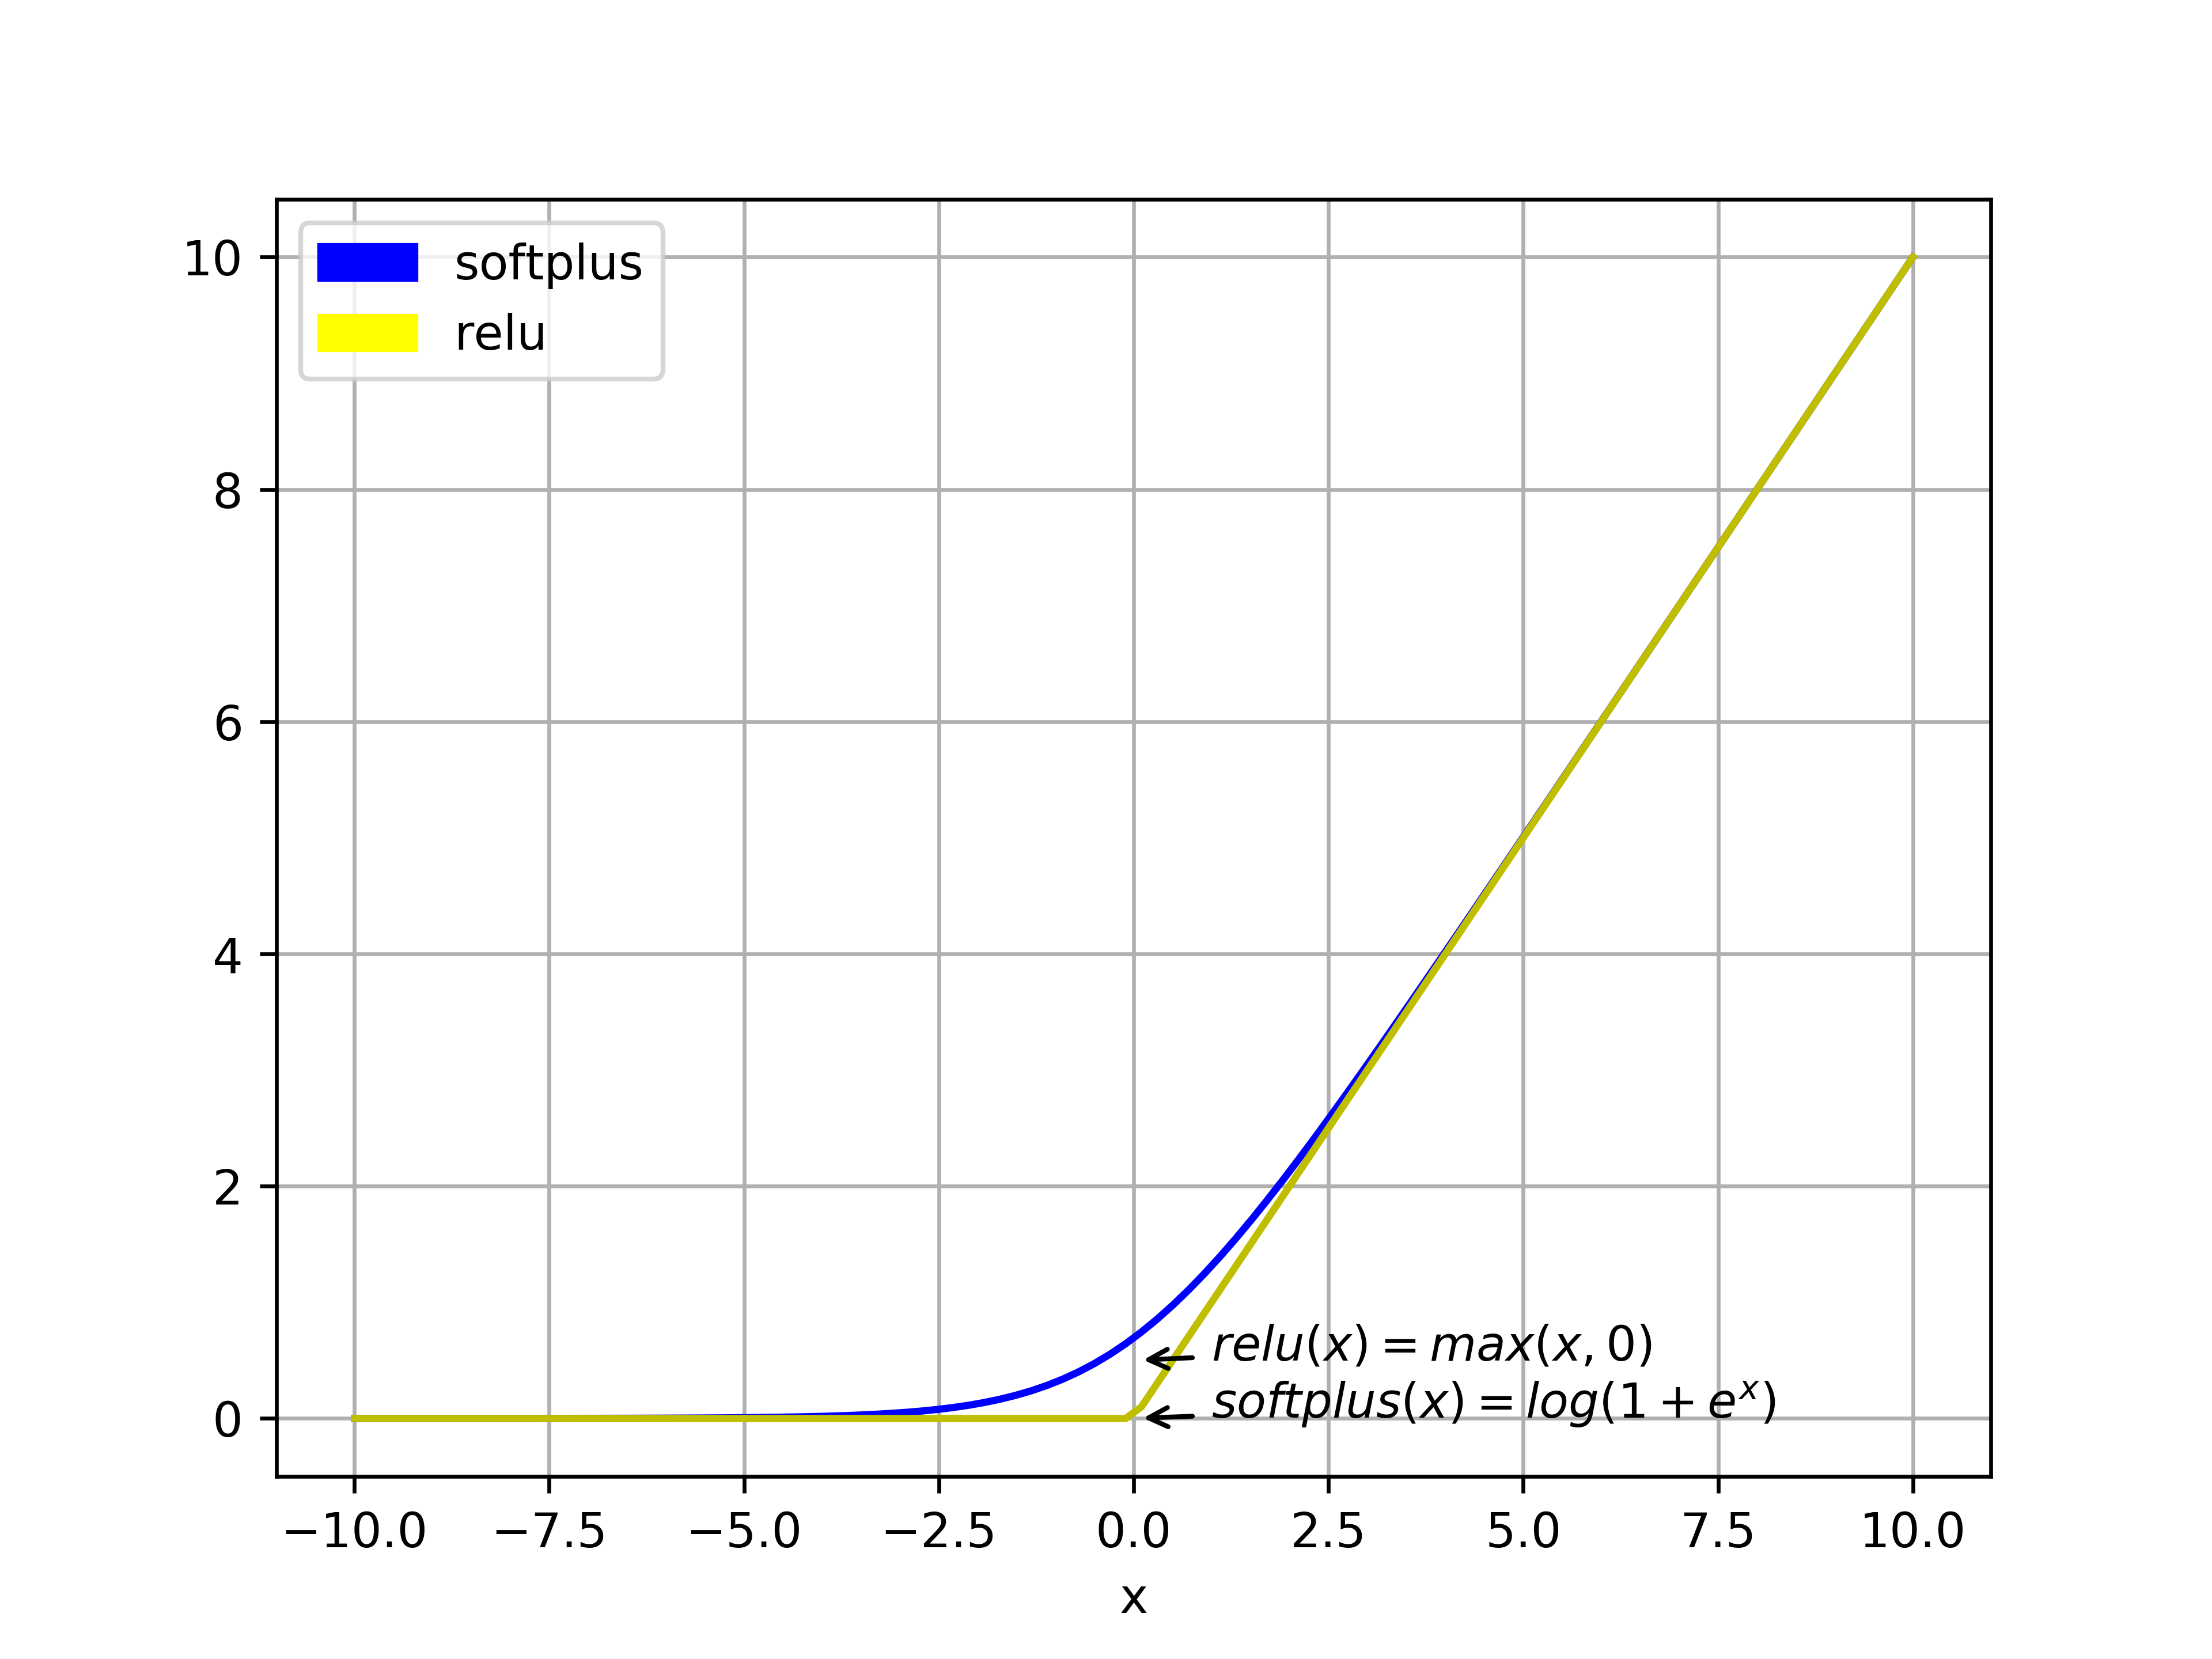
\includegraphics[scale=0.8]{./pic/chapter1/relu_softplus.png}
\end{figure}
\subsection{dropout}
将神经元以概率keep\_prob绝对是否被抑制。如果被抑制该神经元的输出为0如果不被抑制,该神经元的输出将被放大到原来的1/keep\_prop。
默认情况下,每个神经元是否被抑制是相互独立的。但是是否被抑制也可以通过noise\_shape来调节。当noise\_shape[i]=shape(x)[i]时,x中的元素相互独立。如果shape(x)=[k,1,1,n],那么每个批通道都是相互独立的,但是每行每列的数据都是关联的,也就是说要么都为0,要么还是原来的值。
\begin{python}
import tensorflow as tf
a = tf.constant([[-1.,2.,3.,4.]])
with tf.Session() as sess:
    b = tf.nn.dropout(a,0.5,noise_shape=[1,4])
    print(sess.run(b))
    c = tf.nn.dropout(a,0.5,noise_shape=[1,1])
    print(sess.run(c))
\end{python}
[[-2.  0.  0.  8.]]\newline
[[-0.  0.  0.  0.]]\newline
当输入数据特征相差明显时,用tanh效果会很好,但在循环过程中会不断扩大特征效果并显示出来。当特征相差不明显时,sigmoid效果比较好。同时,用sigmoid和tanh作为激活函数时,需要对输入进行规范化,否则激活厚的值全部进入平坦区,隐藏层的输出会趋同,丧失原来的特征表达,而relu会好很多,优势可以不需要输入规范化来避免上述情况。因此,现在大部分卷积神经网络都采用relu作为激活函数。
\section{卷积函数}
tf.nn.conv2d(input,filter,padding,stride=None,diation\_rate=Nonei每name = None,data\_format=None)\newline
\begin{itemize}
\item input:一个tensor,数据类型必须是float32,或者是float64
\item filter:一个tensor,数据类型必须和input相同。
\item strides:一个长度为4的一组证书类型数组,每一维对应input中每一维对应移动的步数,strides[1]对应input[1]移动的步数。
\item padding:有两个可选参数'VALID'(输入数据维度和输出数据维度不同)和'SAME'(输入数据维度和输出数据维度相同)
\item use\_cudnn\_on\_gpu:一个可选的布尔值,默认情况下时True。
\item name:可选,操作的一个名字。
\end{itemize}
\begin{python}
import tensorflow as tf
input_data = tf.Variable(tf.random_normal(shape = [10,9,9,3],mean=0,stddev=1),dtype = tf.float32)
kernel = tf.Variable(tf.random_normal(shape = [2,2,3,2],mean = 0,stddev=1,dtype=tf.float32))

y = tf.nn.conv2d(input_data,kernel,strides=[1,1,1,1],padding='SAME')
init = tf.global_variables_initializer()
with tf.Session() as sess:
    sess.run(init)
    print(sess.run(y).shape)
\end{python}
输出形状为[10,9,9,2]。
\section{池化}
\begin{tabular}{|p{15cm}|l|}
池化函数 &功能\\
\hline
\textcircled{1} tf.nn.avg\_pool(value,ksize,strides,padding,data\_format='NHWC',name =None)&平均池化\\
\textcircled{2} tf.nn.max\_pool(value,ksize,strides,padding,data\_format='NHWC',name =None)&最大池化\\
\textcircled{3} tf.nn.max\_pool\_with\_argmax(input,ksize,strides,padding,Targmax=None,name =None)&最大池化返回最大值的位置\\
\textcircled{4} tf.nn.avg\_pool3d(input,ksize,strides,padding,name =None)&三维状态下的平均池化\\
\textcircled{5} tf.nn.max\_pool3d(input,ksize,strides,padding,name =None)&三维状态下的最大池化\\
\textcircled{6} tf.nn.fractionan\_avg\_pool(value,pooling\_ratio,pseudo\_random=None,overlapping=None,deterministic=None,seed = None,seed2=None,name = None)&三维下的平均池化\\
\textcircled{7} tf.nn.avg\_max\_pool(value,pooling\_ratio,pseudo\_random=None,overlapping=None,deterministic=None,seed = None,seed2=None,name = None)&三维状态下的最大池化\\
\textcircled{8} tf.nn.pool(input,window\_shape,pool\_typing,padding,dilation\_rate = None,strides=None,name=None,data\_format=None)&执行一个N为池化操作。
\end{tabular}
\begin{itemize}
\item value:一个四维Tensor,维度时[batch,height,width,chennels]。
\item ksize:一个长度不小于4的整型数据,每一位上的值对应于输入数据Tensor中每一维窗口对应值。
\item stride:一个长度不小于4的整型列表。该参数指定窗口在输入数据Tensor每一维上的步长。
\item padding:一个字符串,取值为SAME或者VALID。
\item data\_format:NHWC。
\end{itemize}
\section{常见的分类函数}
tf.nn.sigmoid\_cross\_entropy\_with\_logits(logits,targets,name=None)
\begin{itemize}
	\item logits:[batch\_size,num\_classes]
	\item targets:[batch\_size,size]
	\item 输出:loss[batch\_size,num\_classes]
\end{itemize}
最后已成不需要进行sigmoid操作。\par
tf.nn.softmax(logits,dim=-1,name=None):计算Softmax
\[softmax = \frac{x^{logits}}{reduce\_sum(e^{logits},dim)}\]
tf.nn.log\_softmax(logits,dim=-1,name = None)计算log softmax
\[logsoftmax = logits-log(reduce\_softmax(exp(logits),dim))\]
tf.nn.softmax\_cross\_entropy\_with\_logits(\_setinel=None,labels=None,logits=None,dim=-1,name=None)
输出loss:[batch\_size]保存的时batch中每个样本的交叉熵。
tf.nn.sparse\_softmax\_cross\_entropy\_with\_logic(logits,labels,name=None)
\begin{itemize}
	\item logits:神经网络最后一层的结果。
	\item 输入logits:[batch\_size,num\_classes],labels:[batch\_size],必须在[0,num\_classes]
	\item loss[batch],保存的是batch每个样本的交叉熵。
\end{itemize}
\section{优化方法}
\begin{itemize}
	\item tf.train.GradientDescentOptimizer
	\item tf.train.AdadeltaOptimizer
	\item tf.train.AdagradDAOptimizer
	\item tf.train.AdagradOptimizer
	\item tf.train.MomentumOptimizer
	\item tf.train.AdamOptimizer
	\item tf.train.FtrlOptimizer
	\item tf.train.RMSPropOptimizer
\end{itemize}
\subsection{BGD}
BGD(batch gradient descent)批量梯度下降。这种方法是利用现有的参数对训练集中的每一个输入生成一个估计输出$y_i$,然后跟实际的输出$y_i$比较,统计所有的误差,求平均后的到平均误差作为更新参数的依据。啊他的迭代过程是:
\begin{enumerate}
	\item 提取巡检集中所有内容$\{x_1,\ldots,x_n\}$,以及相关的输出$y_i$;
	\item 计算梯度和误差并更新参数。
\end{enumerate}
这种方法的优点是:使用所有数据计算,都保证收敛,并且并不需要减少学习率缺点是每一步需要使用所有的训练数据,随着训练的进行,速度会变慢。那么如果将训练数据拆分成一个个batch,每次抽取一个batch数据更新参数,是不是能加速训练?这就是SGD。
\subsection{SGD}
SGD(stochastic gradient descent):随机梯度下降。这种方法的主要思想是将数据集才分成一个个的batch,随机抽取一个batch计算并更新参数,所以也称为MBGD(minibatch gradient descent)\
SGD在每次迭代计算mini-batch的梯度,然后队参数进行更新。和BGD相比,SGD在训练数据集很大时也能以较快的速度收敛,但是它有两个缺点:
\begin{enumerate}
\item 需要手动调整学习率,但是选择合适的学习率比较困难。尤其在训练时,我们常常想队常出现的特征更新速度快点,队不长出现的特征更新速度慢些,而SGD对更新参数时对所有参数采用一样的学习率,因此无法满足要求。
\item SGD:容易收敛到局部最优。
\end{enumerate}
\subsection{momentum}
Momentum时模拟物理学中的动量概念,更新时在一定程度上保留之前的更新方向,利用当前批次再次微调本次更新参数,因此引入了一个新的变量v,作为前几次梯度的累加。因此,momentum能够更新学习率,在下降初期,前后梯度方向一致时能加速学习:在下降的中后期,在局部最小值附近来回振荡,能够抑制振荡加快收敛。
\subsection{Nesterov Momentum}
标准的Monentum法首先计算一个梯度,然后子啊加速更新梯度的方向进行一个大的跳跃Nesterov首先在原来加速的梯度方向进行一个大的跳跃,然后在改为值设置计算梯度值,然后用这个梯度值修正最终的更新方向。
\subsection{Adagrad}
Adagrade能够自适应的为哥哥参数分配不同的学习率,能够控制每个维度的梯度方向,这种方法的优点是能实现学习率的自动更改,如果本次更新时梯度大,学习率就衰减得快,如果这次更新时梯度小,学习率衰减得就慢些。
\subsection{RMSprop}
和Momentum类似,通过引入衰减系数使得每个回合都衰减一定比例。在实践中,对循环神经网络效果很好。
\subsection{Adam}
名称来自自适应矩阵(adaptive moment estimation).Adam更均损失函数针对每个参数的一阶矩,二阶矩估计动态调整每个参数的学习率。
\begin{python}
import numpy as np
import tensorflow as tf
import matplotlib.pyplot as plt
tf.set_random_seed(0)
np.random.seed(0)
LR = 0.01
BATCH_SIZE = 32
x = np.linspace(-1,1,100).reshape(-1,1)
noise = np.random.normal(0,0.1,size=x.shape)
y = np.power(x,2)+noise
class Net:
    def __init__(self,opt,**kwargs):
        self.x = tf.placeholder(tf.float32,[None,1])
        self.y = tf.placeholder(tf.float32,[None,1])
        l = tf.layers.dense(self.x,20,tf.nn.relu)
        out = tf.layers.dense(l,1)
        self.loss = tf.losses.mean_squared_error(self.y,out)
        self.train = opt(LR,**kwargs).minimize(self.loss)
net_SGD = Net(tf.train.GradientDescentOptimizer)
net_momentum = Net(tf.train.MomentumOptimizer,momentum=0.9)
net_RMSprop = Net(tf.train.RMSPropOptimizer)
net_Adam = Net(tf.train.AdamOptimizer)
nets = [net_SGD,net_momentum,net_RMSprop,net_Adam]
sess = tf.Session()
sess.run(tf.global_variables_initializer())
losses_his = [[],[],[]]
for step in range(300):
    index = np.random.randint(0,x.shape[0],BATCH_SIZE)
    b_x = x[index]
    b_y = y[index]
    for net,l_his in zip(nets,losses_his):
        _,l = sess.run([net.train,net.loss],{net.x:b_x,net.y:b_y})
        l_his.append(l)
labels = ['SGD','Momentum','RMSprop','Adam']
for i,l_his in enumerate(losses_his):
    plt.plot(l_his,label=labels[i])
plt.legend(loc='best')
plt.xlabel('Step')
plt.ylabel('Loss')
plt.ylim(0,0.2)
plt.savefig('Opt.png',dpi=600)
\end{python}
\begin{figure}[H]
	\centering
	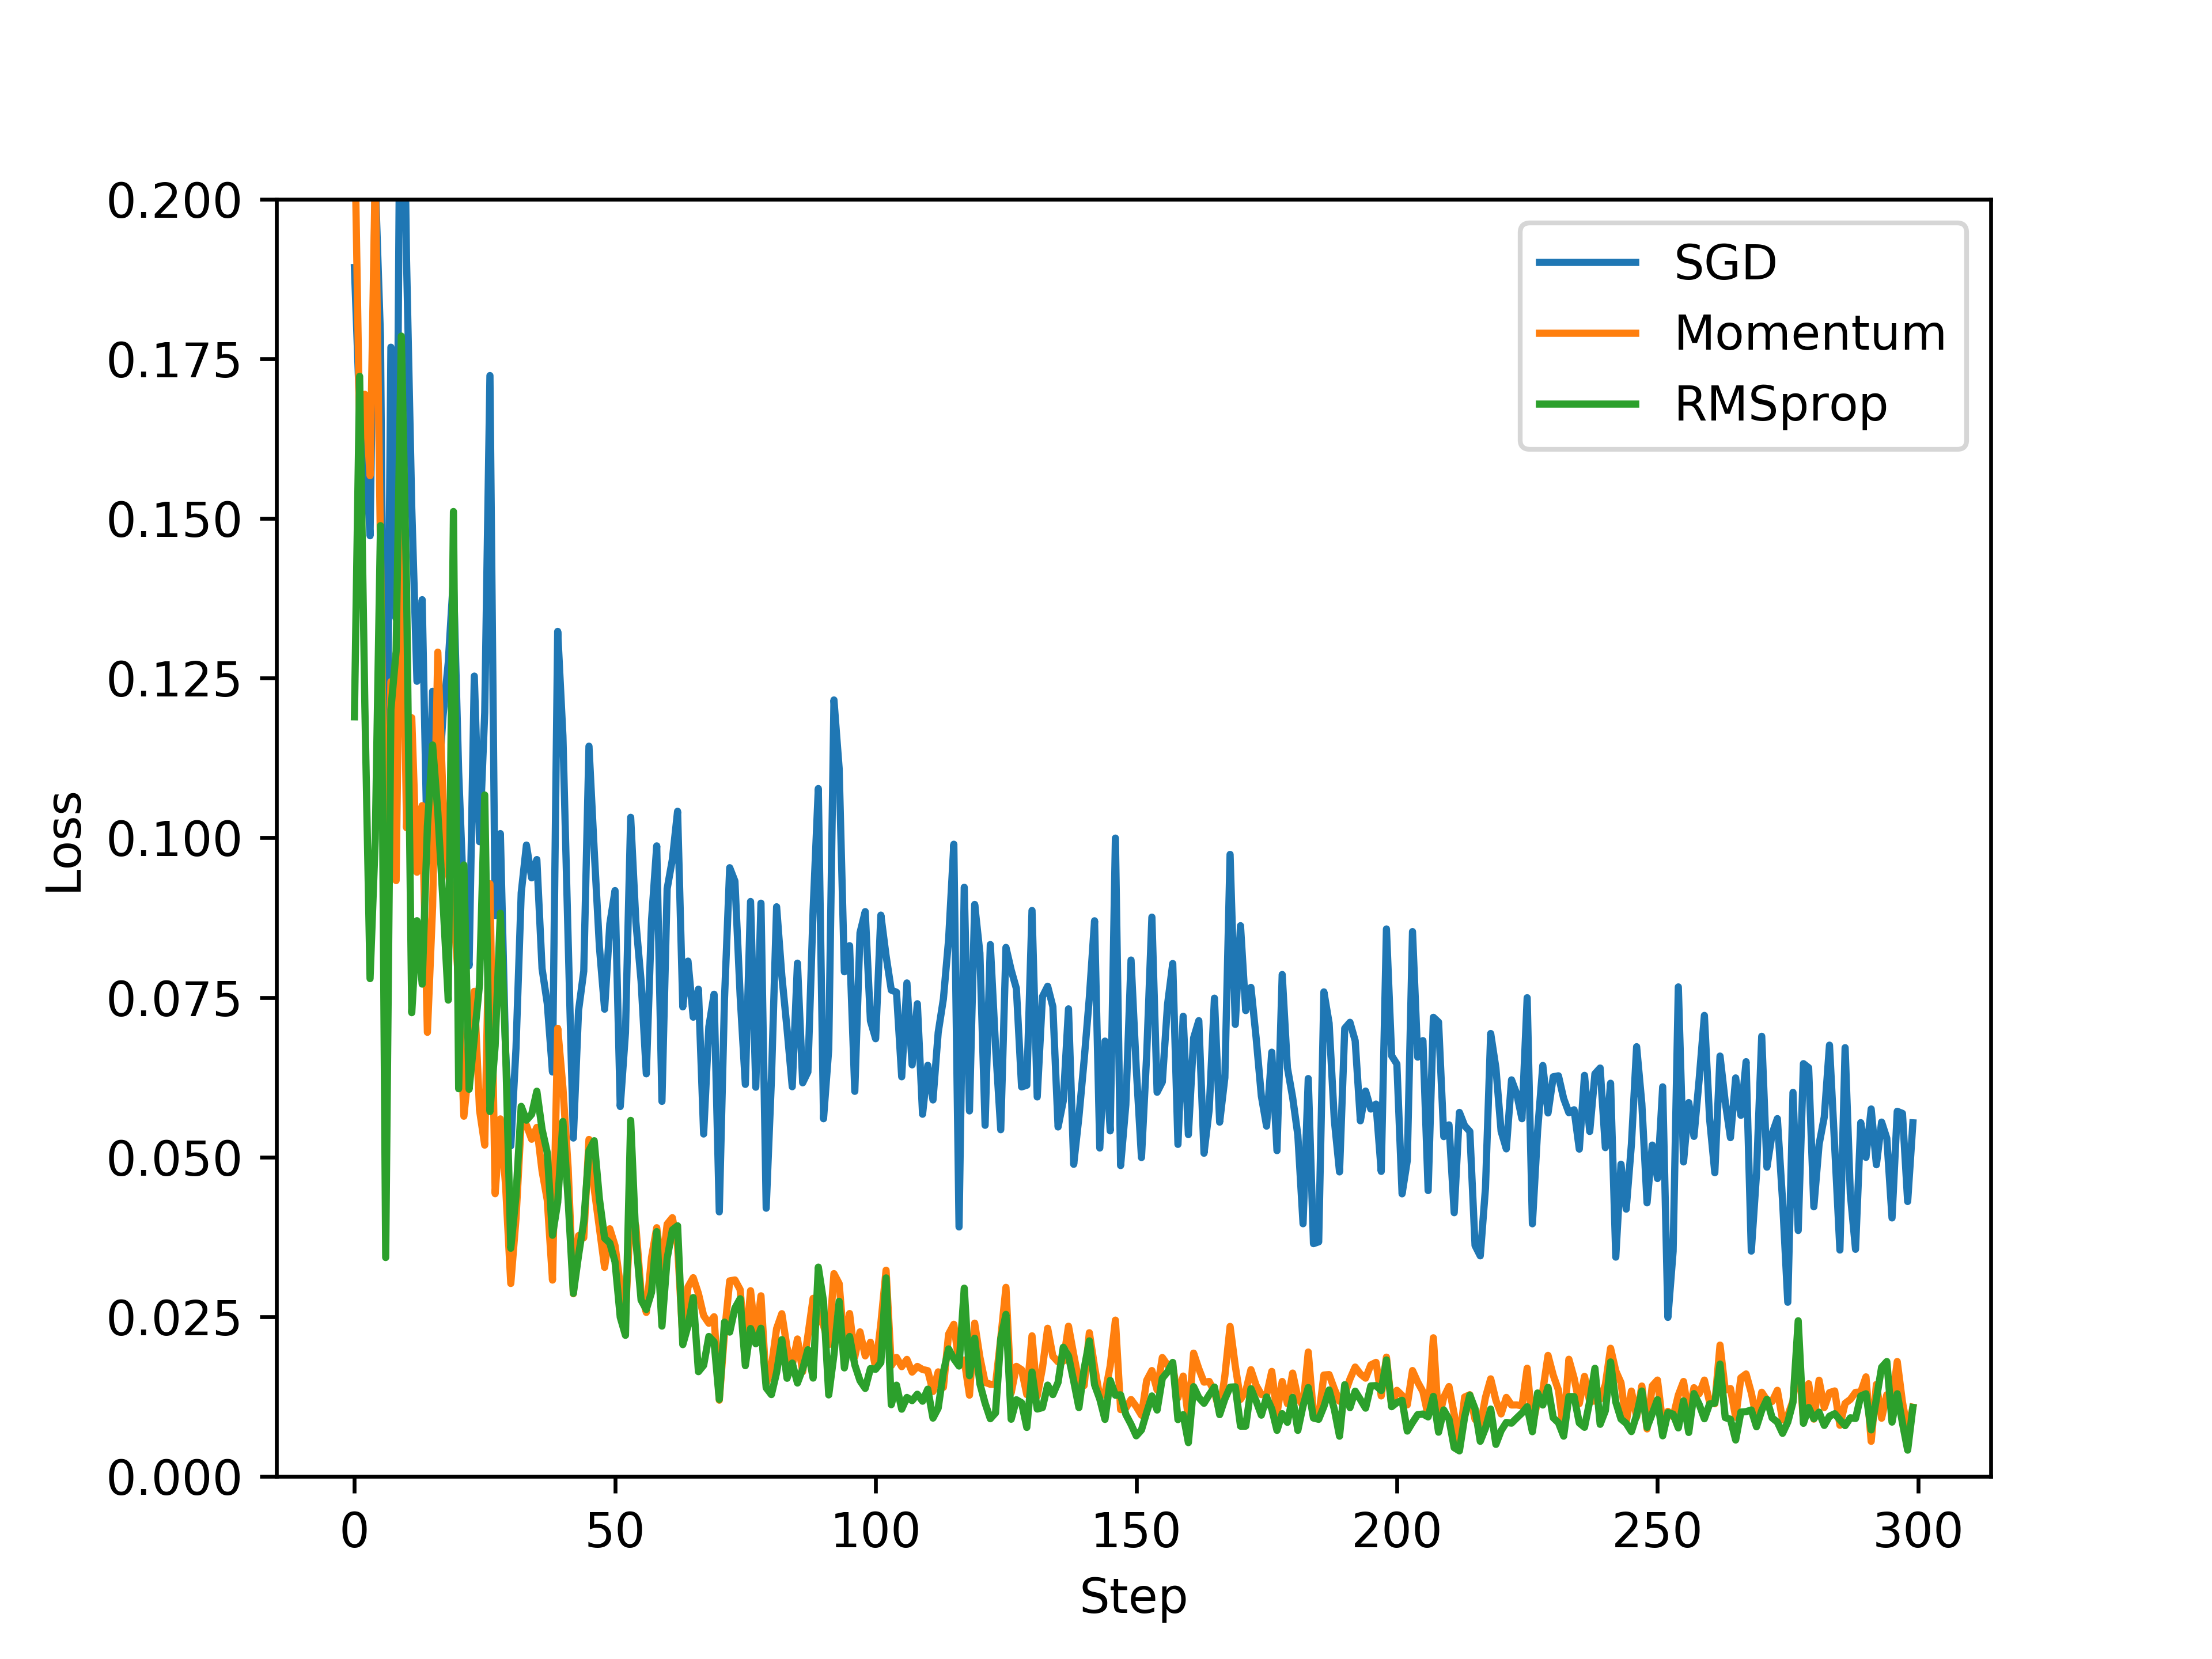
\includegraphics[scale=0.6]{./pic/chapter1/Opt.png}
\end{figure}
\subsection{常用的度量函数tf.metrics}
accuracy(labels,predictions,weights=None,metrics\_collections,updates\_collections=None,name=None)
\begin{itemize}
	\item labels:Tensor,和predictions的形状相同,代表真实值。
	\item predictions:Tensor,代表预测值。
	\item weights:Tensor,rank可以为0或者labels的rank,必须能和label广播(所有的维度必须是1,或者和labels维度相同)
	\item metrics\_collection:accuracy应该被增加的一个collectiobn列表选项。
	\item update\_collections:update\_op应该添加的选项列表。
	\item name:Variable\_scope名字选项。
	\item accuracy:返回值Tensor,代表精度,总共预测对的和总数的商。
	\item update\_op:返回值适当增加total和count变量和accuracy匹配。
	\item ValueError:异常如果predictions和labels有不同的形状,或者weight不是None它的形状不合prediction匹配,或者metrics\_collections会哦这updates\_collections不是一个list或者tuple。
\end{itemize}
\subsection{构造简单的神经网络拟合数据}
原始数据为$y=x^2$的基础上添加随机噪声。原始数据的散点图如下
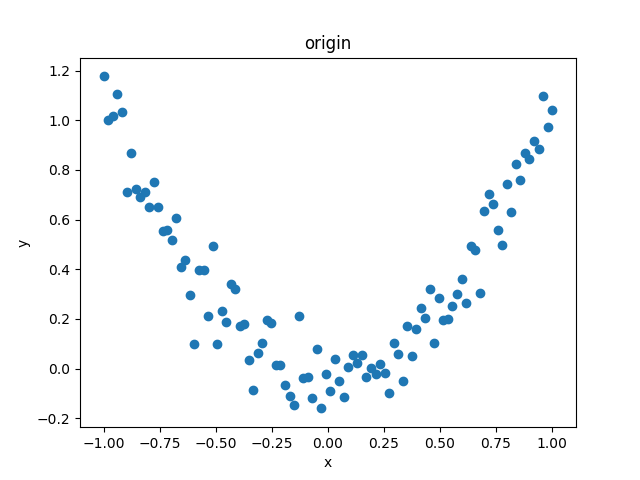
\includegraphics[scale=0.6]{./pic/chapter1/origin.png}
\begin{python}
#tensorflow 1.2.1
import tensorflow as tf
import matplotlib.pyplot as plt
import numpy as np
tf.set_random_seed(0)
np.random.seed(0)
#生成数据
step = 100
x = np.linspace(-1,1,step).reshape(-1,1)
noise = np.random.normal(0,0.1,size=x.shape)
y = np.power(x,2)+noise

tf_x = tf.placeholder(tf.float32,x.shape)
tf_y = tf.placeholder(tf.float32,x.shape)
l1 =  tf.layers.dense(tf_x,10,tf.nn.relu)
output = tf.layers.dense(l1,1)

loss = tf.losses.mean_squared_error(tf_y,output)
optimizer = tf.train.GradientDescentOptimizer(learning_rate=0.5)
train_op = optimizer.minimize(loss)

sess = tf.Session()
sess.run(tf.global_variables_initializer())
plt.ion()
for step in range(100):
    _,l,pred = sess.run([train_op,loss,output],{tf_x:x,tf_y:y})
    if step%5==0:
        plt.cla()
        plt.scatter(x,y)
        plt.title(r'$y=x^2+noise$')
        plt.plot(x,pred,'r-',lw=2)
        plt.text(0,0.8,'Loss=%.4f'%l,fontdict={'size':10,'color':'blue'})
        plt.xlabel("x")
        plt.ylabel(r"$y=x^2$")
        plt.pause(0.1)
plt.ioff()
plt.show()
\end{python}
最终拟合数据:
\begin{figure}[H]
\includegraphics[scale=0.4]{./pic/chapter1/final.png}
\end{figure}
\section{TensorBoard}
\begin{python}
import tensorflow as tf
import numpy as np

tf.set_random_seed(1)
np.random.seed(1)

# fake data
x = np.linspace(-1, 1, 100)[:, np.newaxis]          # shape (100, 1)
noise = np.random.normal(0, 0.1, size=x.shape)
y = np.power(x, 2) + noise                          # shape (100, 1) + some noise

with tf.variable_scope('Inputs'):
        tf_x = tf.placeholder(tf.float32, x.shape, name='x')
        tf_y = tf.placeholder(tf.float32, y.shape, name='y')
with tf.variable_scope('Net'):
    l1 = tf.layers.dense(tf_x, 10, tf.nn.relu, name='hidden_layer')
    output = tf.layers.dense(l1, 1, name='output_layer')
    tf.summary.histogram('h_out', l1)
    tf.summary.histogram('pred', output)
    loss = tf.losses.mean_squared_error(tf_y, output, scope='loss')
    train_op = tf.train.GradientDescentOptimizer(learning_rate=0.5).minimize(loss)
    tf.summary.scalar('loss', loss)     # add loss to scalar summary

    sess = tf.Session()
    sess.run(tf.global_variables_initializer())

    writer = tf.summary.FileWriter('./log', sess.graph)     # write to file
    merge_op = tf.summary.merge_all()                       # operation to merge all summary

    for step in range(100):
        _, result = sess.run([train_op, merge_op], {tf_x: x, tf_y: y})
        writer.add_summary(result, step)
\end{python}
\begin{figure}[H]
	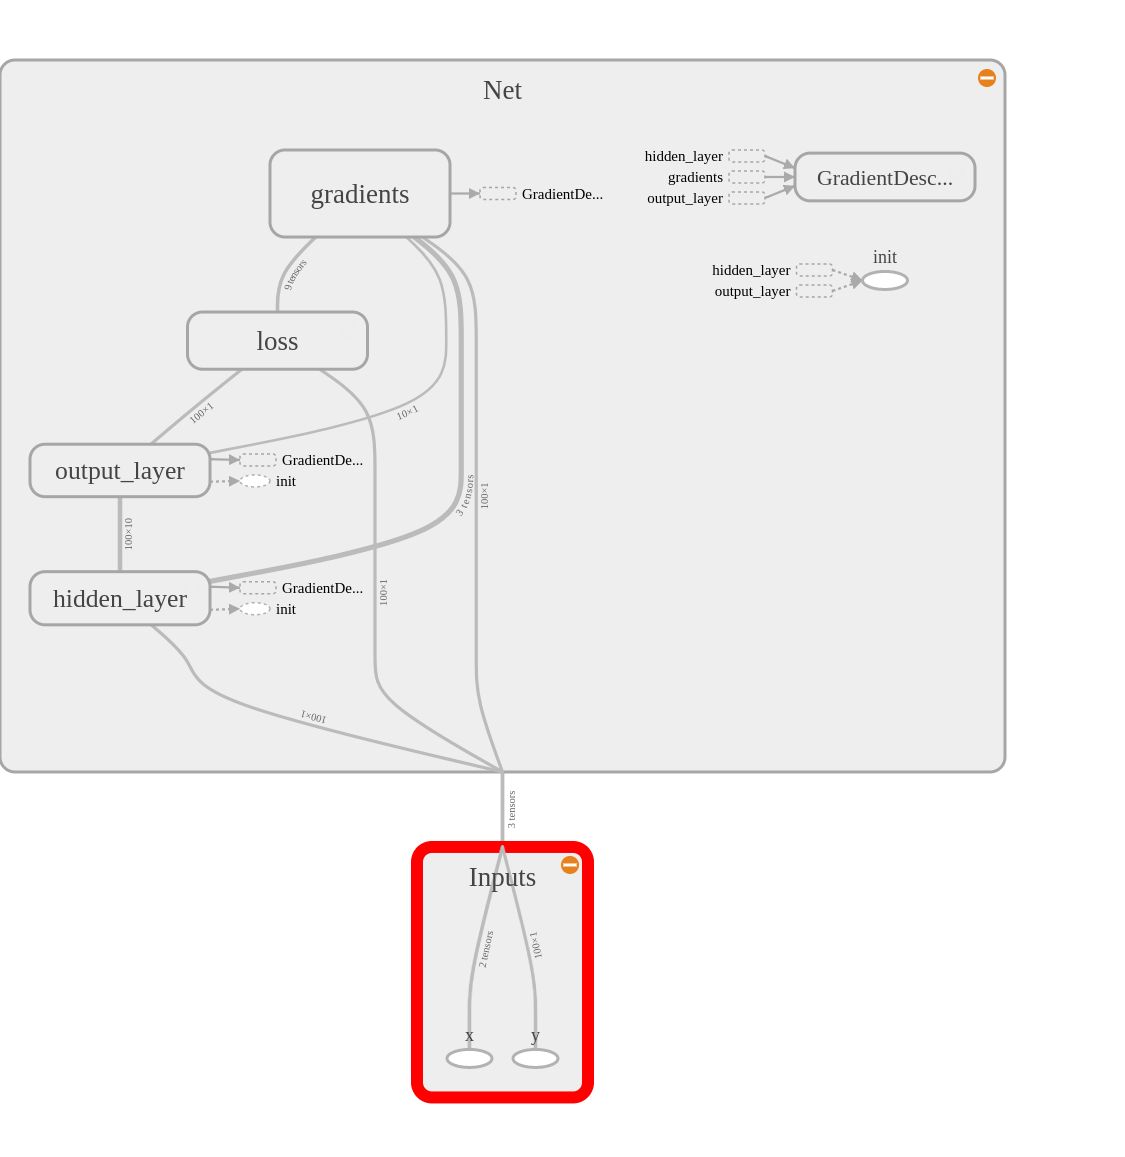
\includegraphics[scale=0.4]{./pic/chapter1/tenbor1.png}
\end{figure}

\chapter{数据的存储和加载}
\begin{python}
import tensorflow as tf
import matplotlib.pyplot as plt
import numpy as np
tf.set_random_seed(0)
np.random.seed(0)
x = np.linspace(-1,1,100).reshape(-1,1)
noise = np.random.normal(0,0.1,size=x.shape)
y = np.power(x,2)+noise
def gendata():
    t = np.linspace(-1,1,100).reshape(-1,1)
def save():
    print('This is save')
    tf_x = tf.placeholder(tf.float32,x.shape)
    tf_y = tf.placeholder(tf.float32,y.shape)
    l = tf.layers.dense(tf_x,10,tf.nn.relu)
    o = tf.layers.dense(l,1)
    loss = tf.losses.mean_squared_error(tf_y,o)
    train_op = tf.train.GradientDescentOptimizer(learning_rate=0.5).minimize(loss)
    sess = tf.Session()
    sess.run(tf.global_variables_initializer())
    saver = tf.train.Saver()
    for step in range(100):
        sess.run(train_op,{tf_x:x,tf_y:y})
    saver.save(sess,'params',write_meta_graph=False)
    pred,l = sess.run([o,loss],{tf_x:x,tf_y:y})
    plt.figure(1,figsize=(10,5))
    plt.subplot(121)
    plt.scatter(x,y)
    plt.plot(x,pred,'r-',lw=5)
    plt.text(-1,1.2,'save loss=%.4f'%l,fontdict={'size':15,'color':'red'})
def reload():
    print('This is reload')
    tf_x = tf.placeholder(tf.float32,x.shape)
    tf_y = tf.placeholder(tf.float32,y.shape)
    l_ = tf.layers.dense(tf_x,10,tf.nn.relu)
    o_ = tf.layers.dense(l_,1)
    loss_ = tf.losses.mean_squared_error(tf_y,o_)
    sess = tf.Session()
    saver = tf.train.Saver()
    saver.restore(sess,'params')
    pred,l = sess.run([o_,loss_],{tf_x:x,tf_y:y})
    plt.subplot(122)
    plt.scatter(x,y)
    plt.plot(x,pred,'r-',lw=5)
    plt.text(-1,1.2,'Reload Loss=%.4f'%l,fontdict={'size':15,'color':'red'})
    plt.show()
save()
tf.reset_default_graph()
reload()
\end{python}
\section{CNN手写体数据识别}
\subsection{mnist数据集}
手写体数据训练集有55000张手写体数据图片。测试集有10000张图片。每张图片是大小为32*32的灰度图片。
卷积神经网络结构:
\begin{itemize}
	\item 第一层卷积层:卷积核16个,卷积核大小为$5\times5$,strides=1,padding为SAME,激活函数为relu(输出大小为$28\times28\times16$)。
	\item 第一层池化层:池化层大小为2,strides为2($14\times14\times16$)。
第二层卷积层:卷积核32,大小为$5\times5$,strides=1,padding为SAME,激活函数为relu。($14\times14\times32$)
	\item 第二层池化层:池化层大小为2,strides为2($7\times7\times32$)。
	\item flatten:1568。
\end{itemize}
\begin{figure}[H]
	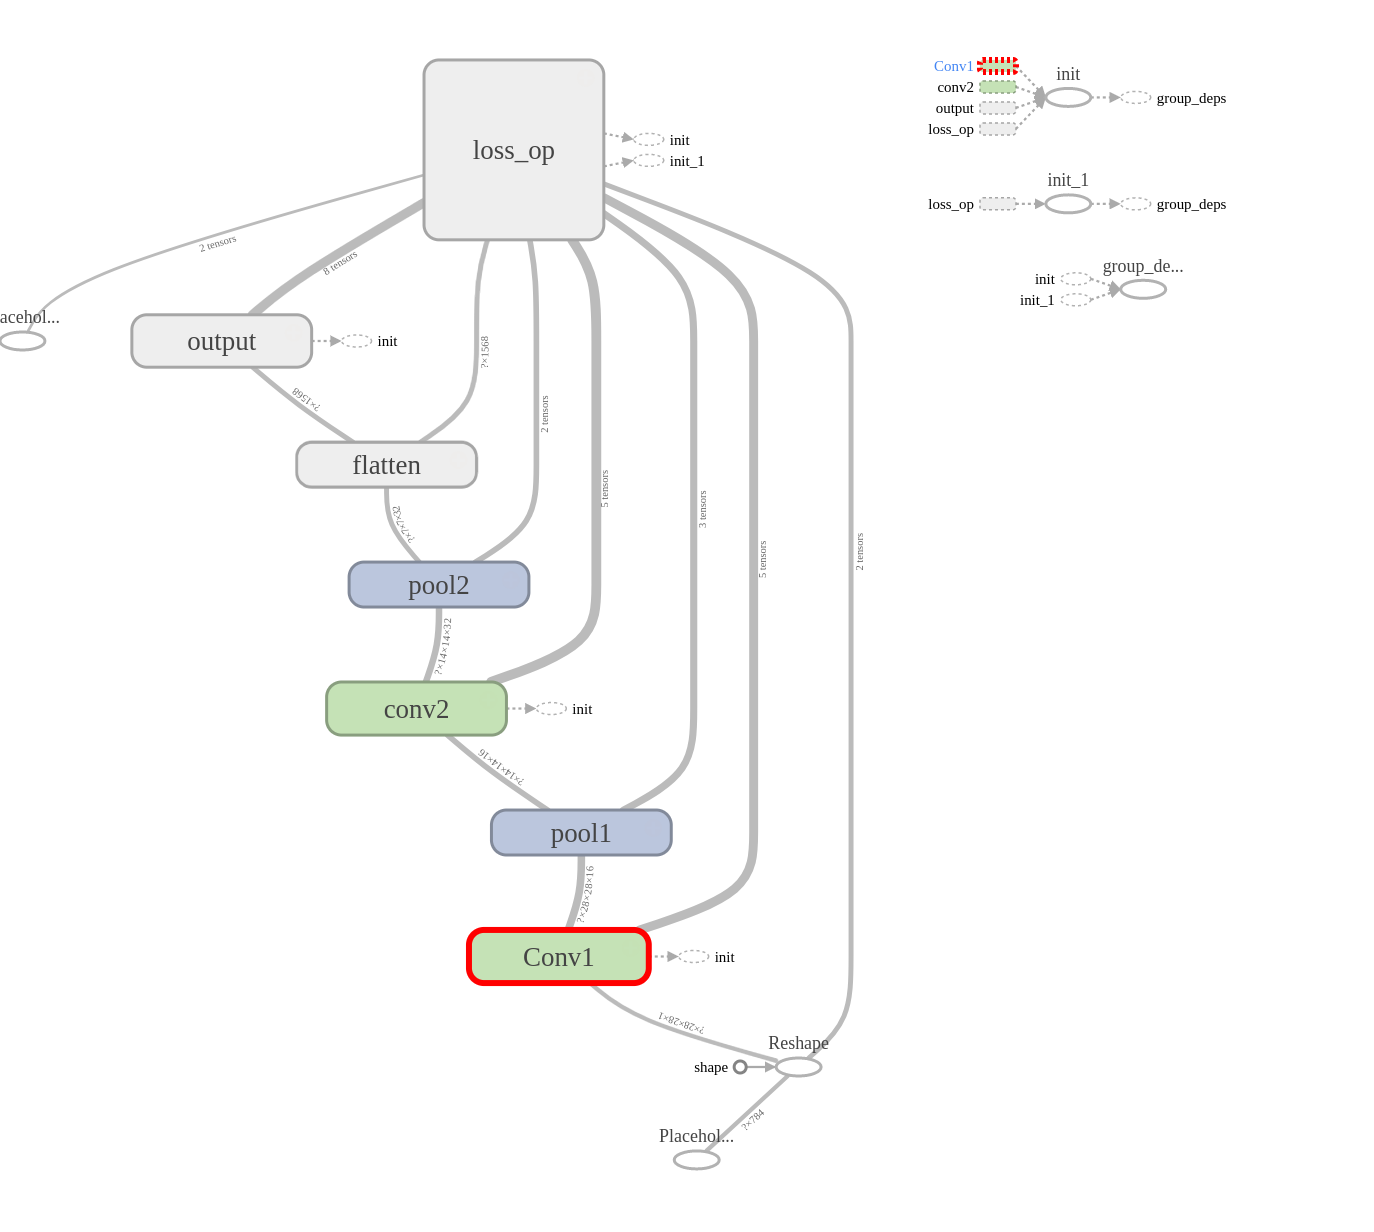
\includegraphics[scale=0.4]{./pic/chapter1/mnist_cnn.png}
\end{figure}
\begin{python}
import tensorflow as tf
import matplotlib.pyplot as plt
import numpy as np
from tensorflow.examples.tutorials.mnist import input_data

tf.set_random_seed(0)
np.random.seed(0)

BATCH_SIZE = 50
LR = 0.001
mnist = input_data.read_data_sets('/home/hpc/文档/mnist_tutorial/mnist',one_hot = True)
test_x = mnist.test.images[:2000]
test_y = mnist.test.labels[:2000]

tf_x = tf.placeholder(tf.float32,[None,28*28])
images = tf.reshape(tf_x,[-1,28,28,1])
tf_y = tf.placeholder(tf.int32,[None,10])
with tf.variable_scope('Conv1'):
    conv1 = tf.layers.conv2d(
            inputs = images,
            filters = 16,
            kernel_size = 5,
            strides = 1,
            padding = 'same',
            activation = tf.nn.relu
        )
    tf.summary.histogram('conv1',conv1)
with tf.variable_scope('pool1'):
    pool1 = tf.layers.max_pooling2d(
            conv1,
            pool_size=2,
            strides =2
        )
    tf.summary.histogram('max_pool1',pool1)
with tf.variable_scope('conv2'):
    conv2 = tf.layers.conv2d(pool1,32,5,1,'SAME',activation=tf.nn.relu)
    tf.summary.histogram('conv2',conv2)
with tf.variable_scope('pool2'):
    pool2 = tf.layers.max_pooling2d(conv2,2,2)
    tf.summary.histogram('max_pool',pool2)
with tf.variable_scope('flatten'):
    flat = tf.reshape(pool2,[-1,7*7*32])
with tf.variable_scope('output'):
    output = tf.layers.dense(flat,10)
with tf.variable_scope('loss_op'):
    loss = tf.losses.softmax_cross_entropy(onehot_labels=tf_y,logits=output)
    train_op = tf.train.AdamOptimizer(LR).minimize(loss)
    accuracy = tf.metrics.accuracy(labels = tf.argmax(tf_y,axis=1),predictions=tf.argmax(output,axis=1),)[1]
    tf.summary.scalar('loss',loss)
    tf.summary.scalar('accuracy',accuracy)
sess = tf.Session()
merge_op = tf.summary.merge_all()
init_op = tf.group(tf.global_variables_initializer(),tf.local_variables_initializer())
sess.run(init_op)
writer = tf.summary.FileWriter('./log',sess.graph)
for step in range(600):
    b_x,b_y = mnist.train.next_batch(BATCH_SIZE)
    _,loss_,result = sess.run([train_op,loss,merge_op],{tf_x:b_x,tf_y:b_y})
    writer.add_summary(result,step)
    if step%50 == 0:
        accuracy_,flat_representation = sess.run([accuracy,flat],{tf_x:test_x,tf_y:test_y})
        print('Step:',step,'| train loss:%.4f'%loss_,'|test accuracy:%.2f'%accuracy_)
test_output = sess.run(output,{tf_x:test_x[:10]})
pred_y = np.argmax(test_output,1)
\end{python}
